Full-stack quality rejection leaves 431 of 437 pairs for inversion; the training branch retains 382 of 393 inputs. The full quality mask accepts 97.02\% of pixels and 99.71\% of the small area's allocated population. Among pixels with matched-input mean support below 0.2, 83.34\% still pass the fixed multi-index mask; the 0.8--1 group has 99.72\% acceptance. Low coherence-screened support is therefore not equivalent to final processing rejection (Fig.~\ref{fig:matched}). Neither acceptance nor rejection is independent physical truth.

At a legacy-support threshold of 0.5, the low-support/accepted and high-support/rejected categories contain 208,609 and 30,637 population allocation units, respectively. That legacy comparison also changes the acquisition period and sample. The matched-input bins provide the within-period comparison: median bootstrap velocity spread is 1.343 versus 1.185 mm yr$^{-1}$ and median inversion residual is 0.673 versus 0.368 mm for the lowest and highest support groups. These associations describe quality differences rather than a binary validity surrogate.

Of 44 excluded pair edges, 44 meet the recorded prediction/reference conditions. Pooled held-out LOS displacement RMSE is 0.984 mm across evaluable observations. Training-mask accepted and rejected locations give 0.699 and 5.150 mm, respectively; the lowest and highest training-support bins give 2.338 and 0.412 mm. On common evaluable observations, time-series differences, training linear velocity and a zero-displacement baseline give 0.984, 11.751 and 11.784 mm. This edge holdout reconstructs pairs between dates already represented in training; shared date-dependent atmospheric phase can also be reconstructed. These are residuals against excluded interferograms with shared acquisitions, not out-of-time forecasts or external velocity accuracies or evidence about permanently missing motion. Exclusions and per-pair results are retained in Supplementary S7.

We additionally compare the same GHSL population field against two distinct support summaries on this processing grid: mean support across the 437 full-stack input pairs and the final LiCSBAS full-stack quality mask. Direct intersections between the native source cells and 1-km UTM cells show that uniform-area allocation increases the mean deficit by 3.066--3.189 percentage points of the fixed AOI population for the 437-pair support field, but by 0.108--0.117 points for the final quality mask across four grid origins. Their native deficits are 3.4539\% and 0.2944\%, respectively. These support definitions carry different processing information; their contrast is not an error comparison, and neither identifies deformation in invalid pixels. The source-to-grid intersections and numerical checks are reported in Supplementary S13.

We also imposed known masks on actual fitted LOS velocities, but only among pixels already accepted by the final quality mask. For a predeclared $-5$ mm yr$^{-1}$ LOS class, 30\% artificial removal and nominal 1.11-km cells, local observed-population prevalence had mean relative bias of +1.1\% under random removal, +5.2\% under clustered removal, $-30.1\%$ when high-spread pixels were preferentially removed, and +79.1\% when low-spread pixels were removed. Nearest-center sampling was much more biased under random removal (+99.7\%). These conditional errors use known velocities in artificially masked valid pixels and do not estimate motion in the original invalid area (Supplementary S14).


\begin{figure}[htbp]\centering
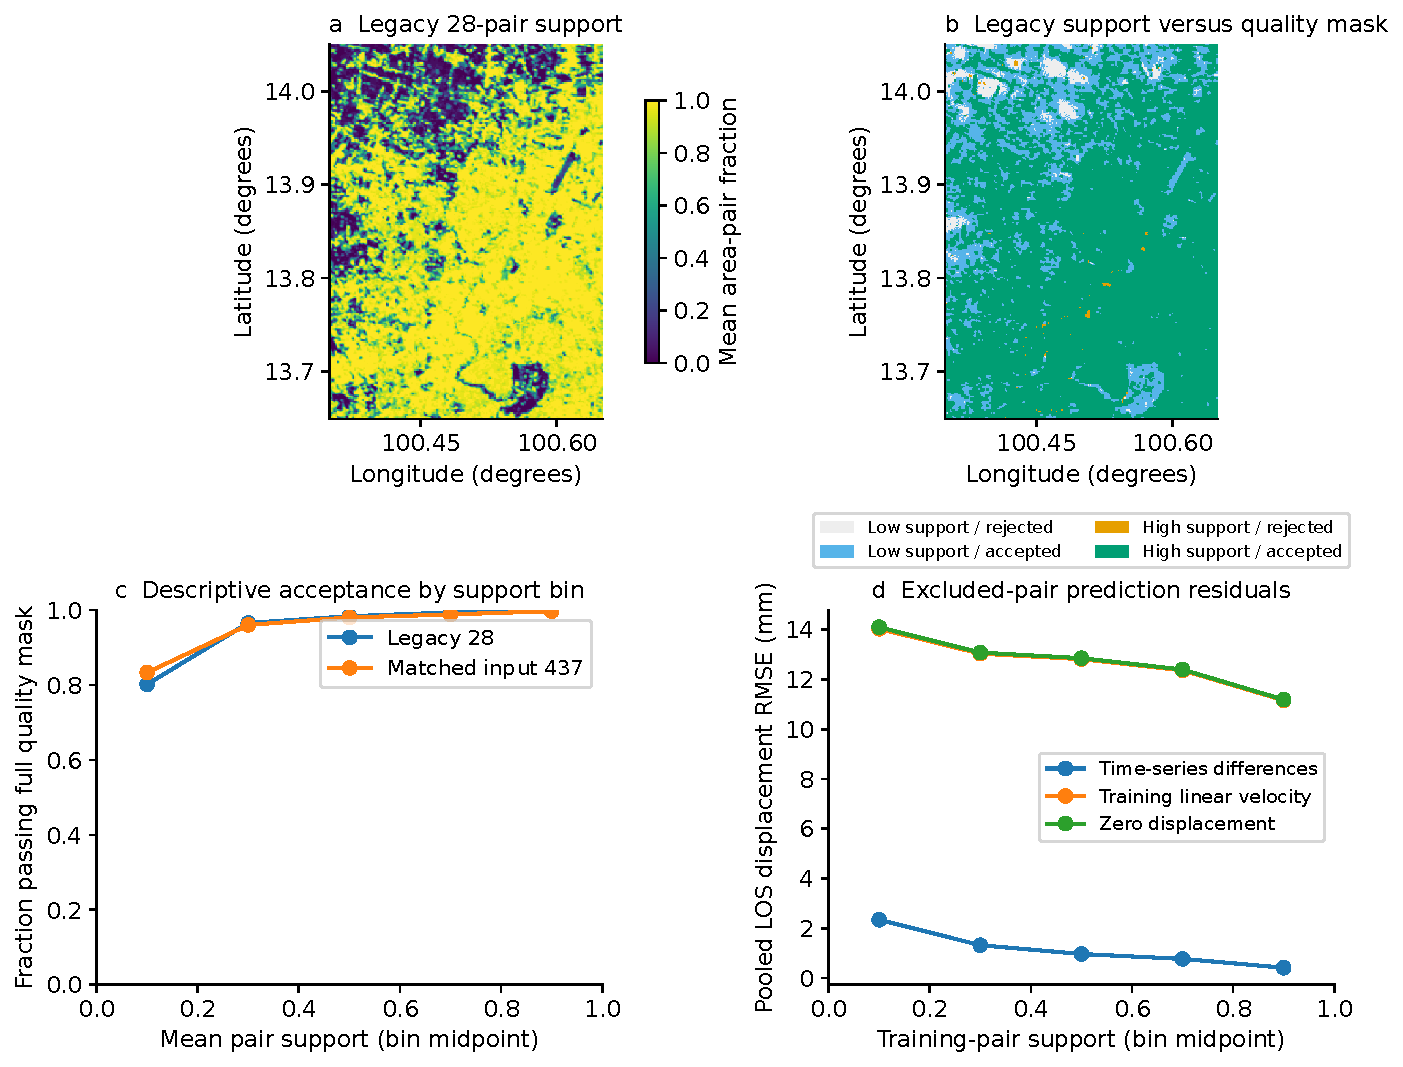
\includegraphics[width=\linewidth]{figures/F7_matched_processing.pdf}
\refstepcounter{figure}\label{fig:matched}
\end{figure}
